\documentclass{beamer}

\usepackage{amsmath, amssymb}
\usepackage{graphicx}
\usepackage[utf8]{inputenc}  % Поддержка UTF-8 кодировки
\usepackage[T2A]{fontenc}    % Кодировка шрифтов для русского языка
\usepackage[english, russian]{babel}  % Подключение русского языка


\title{Neural Operator Search (NOS)}
\author{Терентьев Александр}
\date{\today}

\begin{document}

\frame{\titlepage}

\begin{frame}{Введение}
    \begin{block}{Мотивация}
        Последние достижения в области нейроархитектурного поиска (NAS) позволяют решать сложные задачи, такие как классификация изображений, обнаружение объектов и семантическая сегментация, значительно облегчая требования к знаниям и вмешательству человека за счет автоматизации трудоемкого процесса проектирования нейросетевых архитектур.
    \end{block}
    \begin{itemize}
        \item Поиск архитектуры нейронных сетей — сложная задача.
        \item Стандартные NAS используют ограниченное пространство операций.
        \item Предлагаемый NOS расширяет поиск, включая внимание и динамические свертки.
    \end{itemize}
\end{frame}

\begin{frame}{Постановка задачи}
    \textbf{Определение гетерогенного поискового пространства A:}
    \begin{equation}
        A = Of \cup Oa \cup Od
    \end{equation}
    где:
    \begin{itemize}
        \item \( Of \) – стандартные операции (свертки, пулинг, identity).
        \item \( Oa \) – операции внимания (пространственное, канальное).
        \item \( Od \) – динамические свертки.
    \end{itemize}
\end{frame}

\begin{frame}{Алгоритм NOS}
    \textbf{Формирование выходного признакового тензора:}
    \begin{equation}
        F_{k'} = \sum_{i<k} o_{f}^{i \rightarrow k'} (F_i)
    \end{equation}
    \begin{equation}
        A_{k'} = \sum_{i<k} o_{a}^{i \rightarrow k'} (F_i)
    \end{equation}
    \begin{equation}
    \mathbb{D}_{k'} = \left\{ o_{d}^{i \rightarrow k'} (F_i) \right\}_{i<k}
    \end{equation}
    Расширенная формулировка с вниманием:
    \begin{equation}
        \mathbf{F}_k = \underbrace{\mathbf{F}_k}_{\text{feature}} \oplus \underbrace{(\mathbf{F}_k \odot \mathbf{A}_k)}_{\text{attention}} \oplus \underbrace{\sum_{\mathbf{D}_k \in \mathbb{D}_k} \mathbf{F}_k \otimes \mathbf{D}_k}_{\text{dynamic conv}}
    \end{equation}
\end{frame}

\begin{frame}{Гетерогенная остаточная ячейка}
    \textbf{Структура вычислений:}
    \begin{itemize}
        \item \textbf{Первый уровень} – индивидуальная обработка каждого входного признака, чтобы зафиксировать специфические особенности:
        \begin{equation}
            F_k' = \sum_{i<k} o_{i \to k} (F_i)
        \end{equation}
        \item \textbf{Второй уровень} – коллективное объединение всех входных признаков, чтобы захватить их взаимосвязи:
        \begin{equation}
            F_k = o_{k' \to k} (F_k')
        \end{equation}
    \end{itemize}
    \textbf{Связь между уровнями:}  
    \begin{itemize}
        \item Узел-заместитель \( F'_k \) играет роль промежуточной структуры, связывая два уровня вычислений.
        \item Это позволяет гибко адаптировать входные признаки перед их объединением.
    \end{itemize}
\end{frame}

\begin{frame}{Attention Guided Search (AGS)}
    \textbf{Оптимизация поиска с помощью знания учителя:}
    \begin{equation}
        L_{AT} = \sum_{j \in J} ||vec(\sum_i |F^T_i|^2) - vec(\sum_i |F^S_i|^2)||_2^2
    \end{equation}
    AGS помогает ускорить поиск и улучшить качество найденной архитектуры.
    \begin{figure}
        \centering
        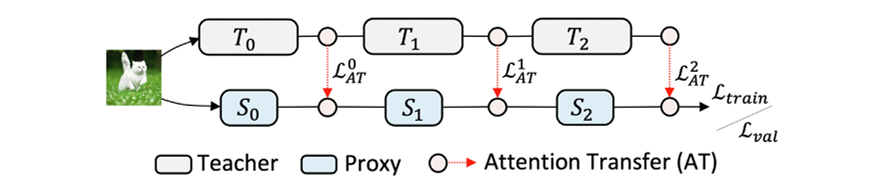
\includegraphics[width=0.8\linewidth]{net.png}
        \caption{Объединенная структура сети учителя-ученика}
        \label{fig:enter-label}
    \end{figure}
\end{frame}

\begin{frame}{Функция потерь}
    \textbf{Оптимизация в NOS включает два уровня:}
    \begin{itemize}
        \item \textbf{Оптимизация параметров нейросети} \( \Theta \):
        \begin{equation}
            \Theta^* = \arg \min_{\Theta} L_{\text{train}}(\Theta, A) + \lambda L_{\text{AT}}(\Theta, A)
        \end{equation}
        \item \textbf{Оптимизация архитектуры сети} \( A \):
        \begin{equation}
            A^* = \arg \min_A L_{\text{val}}(\Theta^*, A) + \lambda L_{\text{AT}}(\Theta^*, A)
        \end{equation}
    \end{itemize}
    где:
    \begin{itemize}
        \item \( L_{\text{train}} \) — функция потерь на обучающем наборе данных.
        \item \( L_{\text{val}} \) — функция потерь на валидационном наборе данных.
        \item \( L_{\text{AT}} \) — дополнительный штраф, учитывающий внимание учителя (teacher network).
        \item \( \lambda \) — коэффициент весового регулирования внимания.
    \end{itemize}
\end{frame}





\begin{frame}{Результаты экспериментов}
    \textbf{Сравнение моделей:}
    \begin{itemize}
        \item CIFAR-10: Ошибка NOS – 2.53% (меньше, чем у DARTS и GDAS).
        \item CIFAR-100: Ошибка NOS – 16.21% (лучше существующих методов).
        \item ImageNet: Высокая эффективность при 440M FLOPs.
    \end{itemize}
    \begin{equation}
        \text{Test Error (\%)} = 2.53 \text{ (CIFAR-10)}, \quad 16.21 \text{ (CIFAR-100)}
    \end{equation}
    \begin{figure}
        \centering
        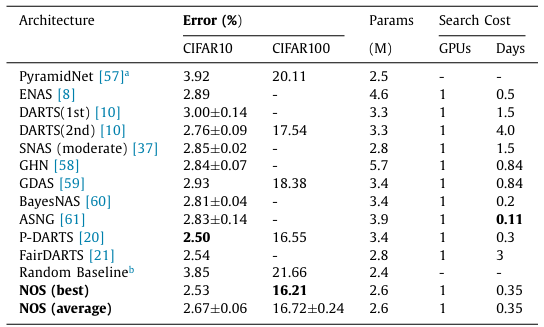
\includegraphics[width=0.5\linewidth]{results.png}
        \caption{Сравнение с современными архитектурами, полученными с помощью прокси-методов NAS на CIFAR10 и CIFAR100 с коэффициентом ошибок Top-1 ( \% ).}
        \label{fig:results}
    \end{figure}
\end{frame}

\begin{frame}{Выводы}
    \begin{itemize}
        \item NOS расширяет пространство поиска архитектуры нейросетей.
        \item Включение внимания и динамических свёрток улучшает обучаемость.
        \item Метод AGS повышает эффективность поиска.
        \item NOS превосходит существующие NAS-методы на нескольких задачах.
    \end{itemize}
\end{frame}

\end{document}